\section{Preliminaries}
\label{preliminaries}
\paragraph{Definition of Agent-Oriented Planning}

In this study, a multi-agent system involves a series of LLM-empowered agents for solving real-world problems.
These agents are constructed by providing specialized tools and unique system prompts that set their identities and instructions, and are powered by LLMs for query understanding, tool use, and response generation.
For example, a search agent can utilize search engines to retrieve up-to-date information relevant to a given query, while a code agent is capable of generating code and executing via a code interpreter.
The collaboration among these agents is facilitated by a meta-agent, which serves as the brain of the multi-agent system.
When a user query is submitted, the meta-agent sends the relevant requests to the appropriate agents, optimizing for both effectiveness and efficiency. The responses produced by these agents are finally aggregated and synthesized to generate a comprehensive answer to the original user query.

Formally, given a user query $Q$, a meta-agent $\mathcal{P}$ needs to select a set of appropriate agents from a total of $n$ agents, denoted as $\mathcal{A}=\{\mathcal{A}_1, ..., \mathcal{A}_n\}$. Each agent is associated with a description $d$ that outlines its capability. We denote the collection of all agent descriptions as $\mathcal{D} = \{d_1,...,d_n\}$.
The user query $Q$ can be decomposed by $\mathcal{P}$ into $m$ sub-tasks, with each sub-task assigned to a specific agent based on their descriptions: 
\begin{equation}
    \mathcal{P}(Q, \mathcal{D}, \mathcal{A})=\{(q_i, \mathcal{A}_i')\ |\ i \in [m]\}. 
\end{equation}
After that, each selected agent $i \in [m]$ produces a response to its assigned sub-task, denoted as $r_i=\mathcal{A}'_i(q_i) $. These responses $\{r_1,...,r_m\}$ are then utilized to generate the final answer to resolve the original query $Q$. 
Such a process is called {\it agent-oriented planning}.

\paragraph{Challenges}
The challenges of agent-oriented planning in multi-agent systems can be two-fold. Firstly, different from existing studies focused on task decomposition~\citep{shen2024hugginggpt, lu2024chameleon} or chain-of-thought reasoning~\citep{wei2022chain}, agent-oriented planning requires intentional decomposition of user queries to effectively associate sub-tasks with agents, which includes considerations of the description of sub-tasks, the granularity of decomposition, the format of the responses, and so on. An example is illustrated at the higher left of Figure~\ref{fig:examples}. 
Given a user query ``How much tin (kg) with 100 kg copper can lower the mixture's melting point to $800\ \tccentigrade$?'', a naive decomposition might suggest ``Determine the melting point of tin and copper'' followed by ``Calculate the amount of tin (kg) required to reduce the melting point of the mixture to $800\ \tccentigrade$ with 100 kg copper''. However, when the sub-task of determining the melting points is assigned to a search agent, it may not result in satisfied responses since the query involves two entities simultaneously. In the context of agent-oriented planning, it is important to consider the capabilities of agents. As a result, such a sub-task should be further decomposed into individual entity searches, i.e., first determine the melting point of tin and then determine the melting point of copper.


Secondly, assigning sub-tasks to appropriate agents is non-trivial, as the meta-agent can only rely on the agents' descriptions to determine task allocation in most cases~\citep{shen2024hugginggpt}. However, a concise and highly generalized description that adequately illustrates an agent's capabilities may not always be available, leading to suboptimal allocation.
For example, if the description of a commonsense agent does not specify the extent of its knowledge base, the meta-agent may struggle to ascertain whether it is suitable to assign the sub-task of querying the melting points of tin and copper to that agent, as shown at the lower left of Figure~\ref{fig:examples}.

\paragraph{Design Principles}
We further identify three critical principles that guide the design of \name for effective and efficient agent-oriented planning in multi-agent systems:
\begin{itemize}
    \item {\it Solvability}. Each sub-task $q_i, \ \forall i \in [m]$ should be independently and completely resolvable by at least one single agent within the multi-agent system, ensuring that the response for each sub-task can be reliable. If a sub-task does not satisfy solvability, the meta-agent is expected to take some modifications or further decomposition.
    \item {\it Completeness}. The array of sub-tasks $\{q_1,...,q_m\}$ should include all necessary information from the original user query $Q$, which ensures that the aggregation of responses of these sub-tasks can effectively yield a comprehensive answer to the user query. 
While a sub-task might include only part of the necessary information, it is not allowable for any particular piece of critical information to be omitted from all sub-tasks.
    \item {\it Non-Redundancy}. The array of sub-tasks $\{q_1,...,q_m\}$ should not include redundant elements, avoiding those task executions that are either irrelevant to resolving $Q$ or duplicated. The principle of non-redundancy promotes that the sub-tasks form a minimal effective set necessary to address the user query, enhancing overall efficiency.
\end{itemize}

Several examples are provided on the right side in Figure~\ref{fig:examples} for a better understanding of these design principles.
Note that here we focus on the redundancy between sub-tasks that should be simplified, and believe that adding redundancy among agents is necessary for fault tolerance as discussed in Appendix~\ref{app: fault_tolerance_agent_availability}, especially considering unexpected changes in agent availability.


While these principles may appear general in nature, we propose an explicit specification and systematic design that follows these principles in the domain of LLM-based multi-agent systems. We hope that these principles, along with the framework we have outlined in the next section, can serve as a good starting point and inspire further research in this field. 


\begin{figure}[!t]
\centering
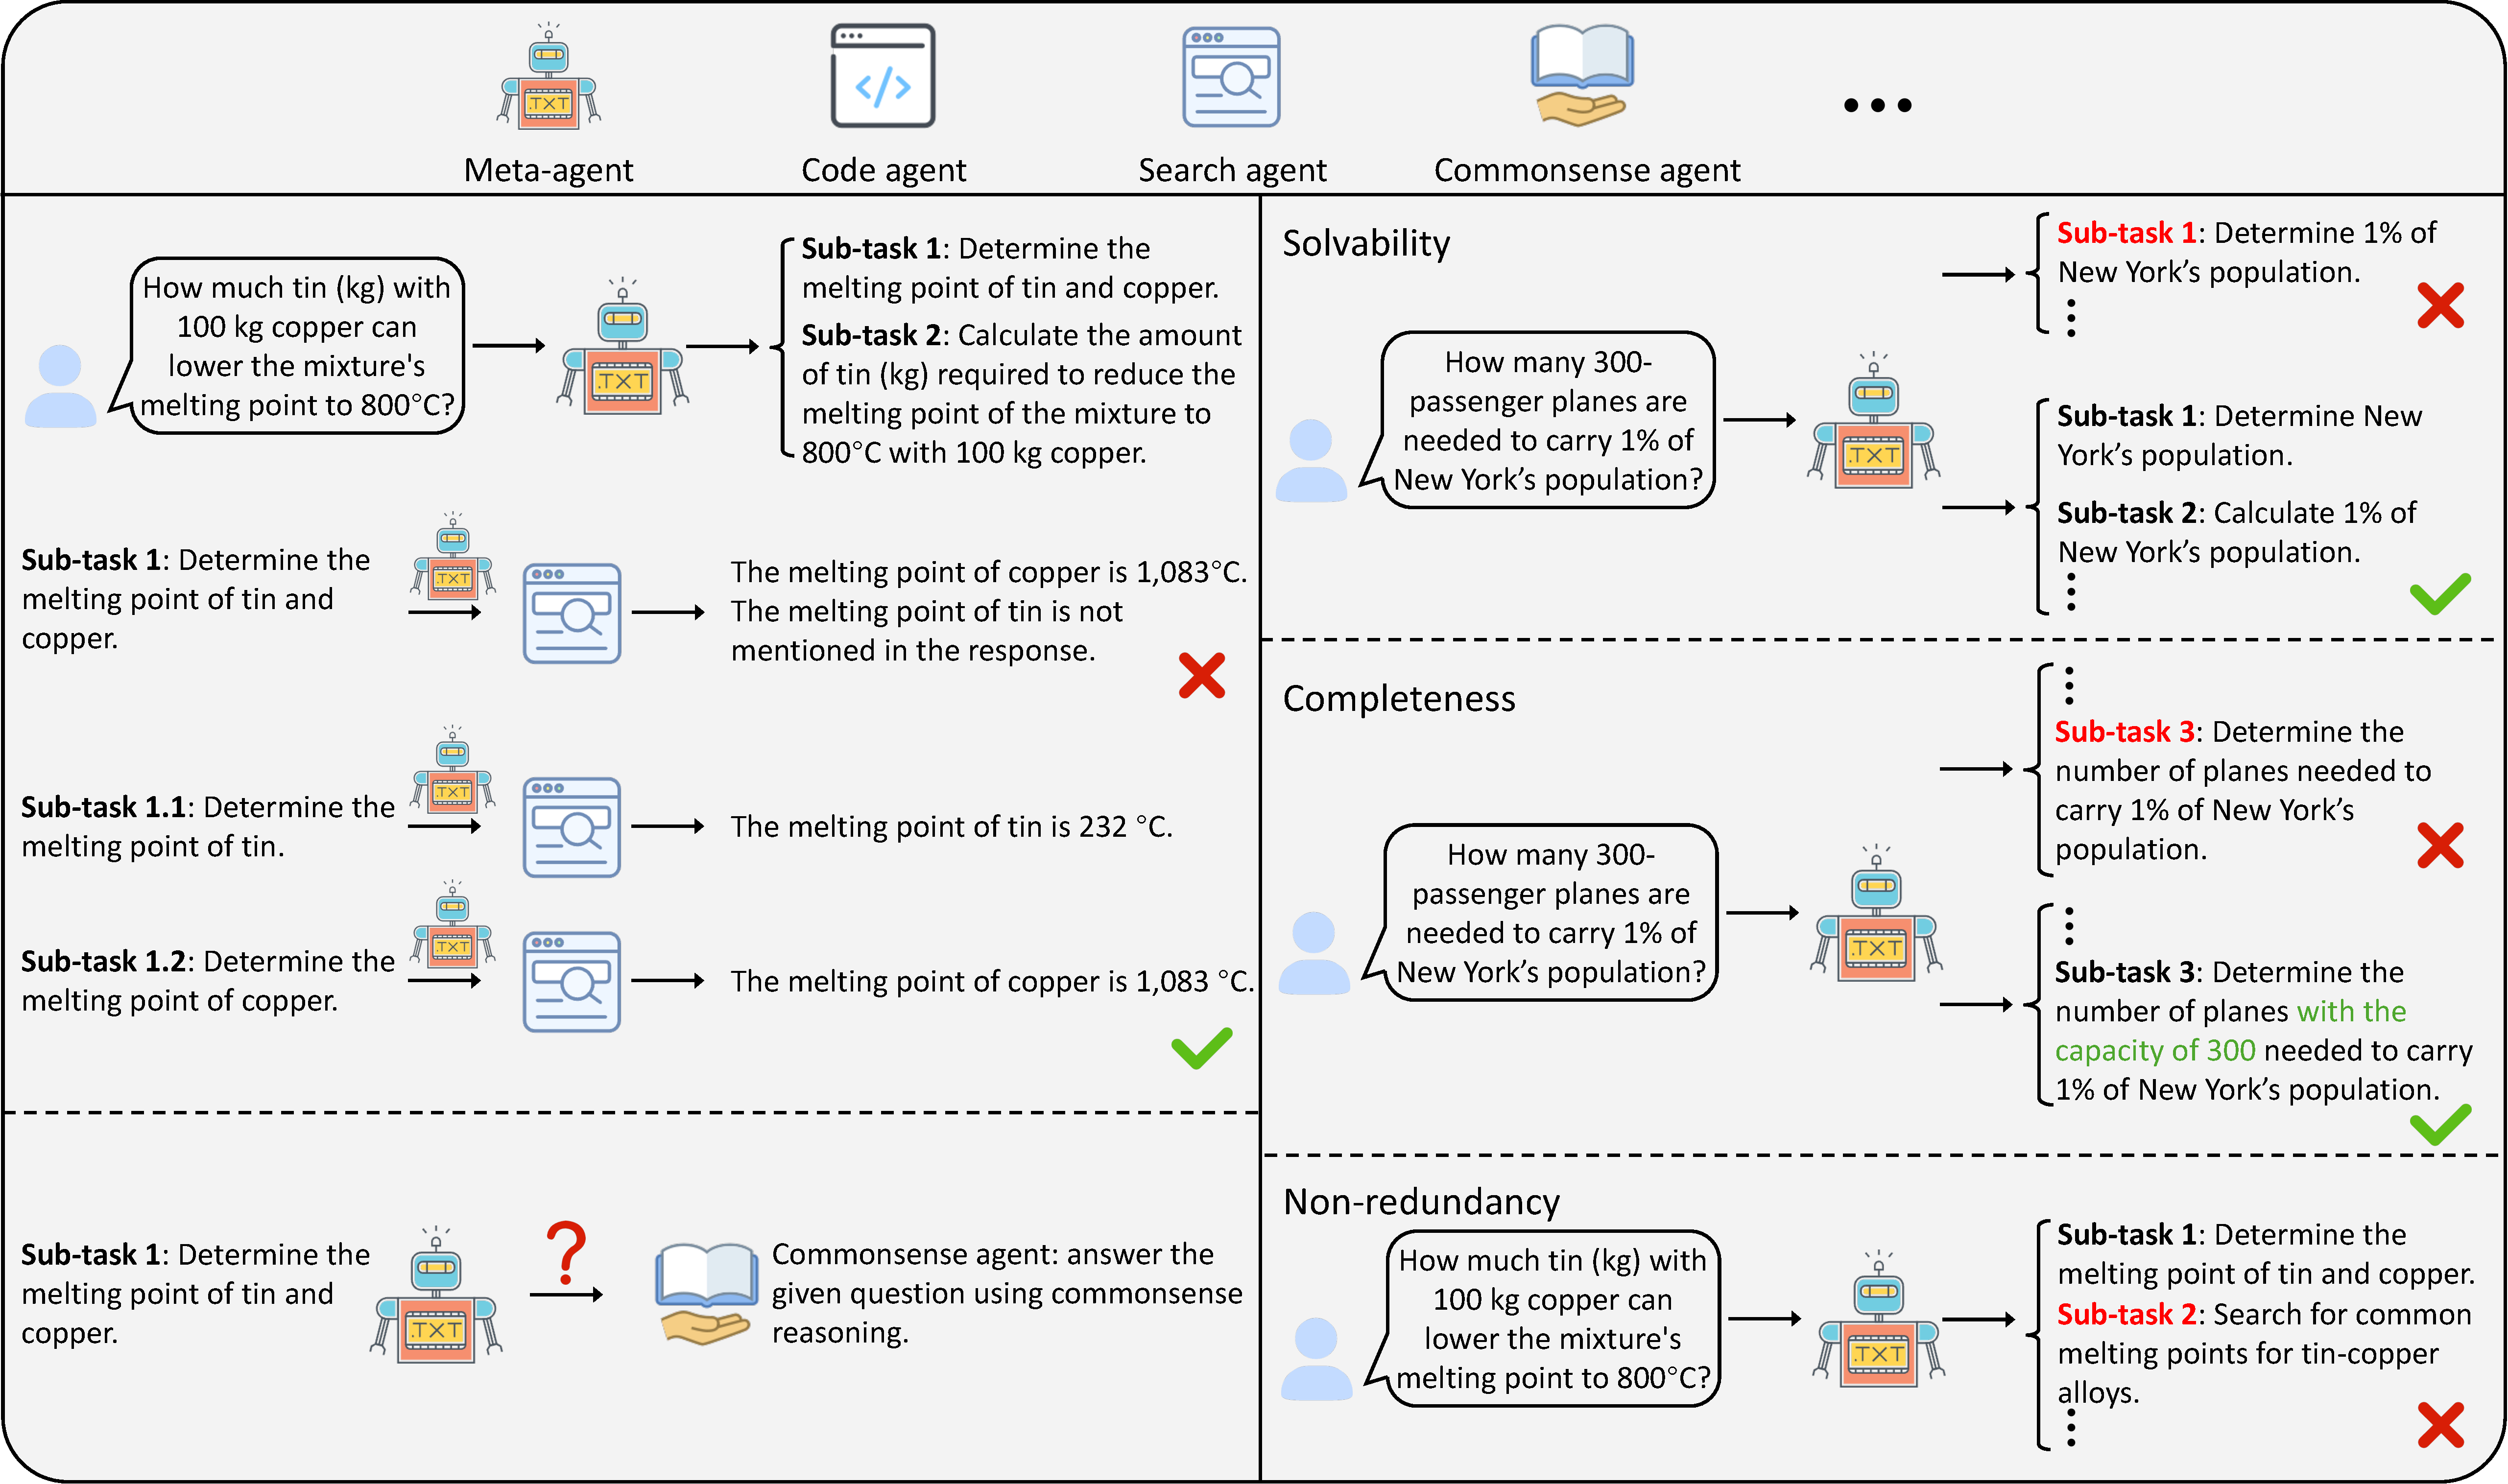
\includegraphics[width=1\linewidth]{figure/challenges.pdf}
\caption{Examples of agent-oriented planning in multi-agent systems, regarding two challenges (left side) and three design principles (right side).}
\label{fig:examples}
\end{figure}



